\documentclass[11pt]{article}
\usepackage[margin=2.3cm]{geometry}
\usepackage{amsmath,amssymb,amsthm,booktabs,graphicx}
\usepackage[colorlinks=true,allcolors=blue]{hyperref}
\usepackage{xurl}

\newcommand{\R}{\mathbb{R}}
\newcommand{\E}{\mathbb{E}}
\newcommand{\hypF}[2]{{}_{#1}F_{#2}}
\newcommand{\file}[1]{\nolinkurl{#1}}
\newcommand{\status}[1]{\textsf{[#1]}}
\newtheorem{theorem}{Theorem}

\title{Notes: when does a Bayesian posterior learn a weak feature?\\[2pt]\large Finite-$n$ transitions in reduced-rank regression}
\author{Francis Headley}
\date{18 October 2026}

\begin{document}
\maketitle

\noindent These notes collect the reduced-rank part of the project.
Statements carry a label: \status{proved} (with the file holding the proof), \status{numerical} (with the check), or \status{heuristic}.
Extensions beyond reduced-rank regression are not included here.

\section{Setting and the question}

Data are $n$ i.i.d.\ pairs with $y=f(x)+\varepsilon$, $\varepsilon\sim\mathcal N(0,1)$, and a model $f_w$ with prior $\varphi(w)$.
The excess loss is $K(w)=\tfrac12\lVert f_w-f\rVert^2$ with $\lVert h\rVert^2=\E_qh(x)^2$.
I work with the population evidence and free energy,
\begin{equation}
  Z_n(f)=\int e^{-nK(w)}\varphi(w)\,dw,\qquad F_n(f)=-\log Z_n(f),
  \label{eq:Z}
\end{equation}
and with sampled data where stated.
For fixed $f$, $F_n=\lambda\log n-(m-1)\log\log n+O(1)$, with learning coefficient $\lambda$ and multiplicity $m$~\cite{Wat09}.

A weak feature is a decomposition $f=f_0+\delta g$, $\lVert g\rVert=1$, where $f_0$ is computed on a larger, more singular set, so that $\lambda_0=\lambda(f_0)<\lambda_1=\lambda(f)$.
Ignoring the feature costs $\Delta L=\delta^2/2$ per sample, and the signal-to-noise ratio is $s=n\Delta L=n\delta^2/2$.

A phase $\alpha$ with local free energy $F_\alpha=nL_\alpha+\lambda_\alpha\log n+c_\alpha$ overtakes another when $n\Delta L+\Delta\lambda\log n+\Delta c=0$~\cite{CLMWM23}.
Dropping $\Delta c$ gives the criterion
\begin{equation}
  n\,\Delta L=\Delta\lambda\,\log n ,
  \label{eq:rule}
\end{equation}
which originates in Sec.~7.6 of Ref.~\cite{Wat09} and is applied to stagewise learning in Refs.~\cite{CHFM25,LUWMW25}.
It predicts that the feature is learned only once $s$ exceeds $\Delta\lambda\log n$.
The question is whether that is right.

To decide when the feature is learned I use a posterior mass: the probability that the fitted amplitude $\alpha$ along $g$ lies within $\delta/2$ of $\delta$.
This window marker vanishes at $s=0$.
It measures the projection along the feature, not the full function error.
The effective learning coefficient $\lambda_n=n\langle K\rangle$ is not used as a marker, because it rises with $s$ before the posterior moves.

\section{One hidden unit: an exact example}

Take $f_w(x)=a\,b^\top x$ with $x\sim\mathcal N(0,I_M)$, standard Gaussian priors, and truth $f(x)=c^\top x$ with $\lvert c\rvert=\delta$, so $f_0=0$, $\lambda_0=\tfrac12$, $\lambda_1=M/2$.
Completing the square in $b$ gives \status{proved, exact}
\begin{equation}
  Z_n=\int\varphi(a)\,(1+na^2)^{-M/2}\,e^{-s/(1+na^2)}\,da .
  \label{eq:toyZ}
\end{equation}
At fixed $s$ the integrand sits at $a=O(n^{-1/2})$, where $\varphi(a)\to\varphi(0)$.
Substituting $t=\sqrt n\,a$ removes $n$ from everything but an overall factor:
\begin{equation}
  F_n=\tfrac12\log n-\log G_M(s)+O(1),\qquad G_M(s)=\int(1+t^2)^{-M/2}e^{-s/(1+t^2)}\,dt .
  \label{eq:toyF}
\end{equation}
Since $G_M(s)=\mathrm B(\tfrac{M-1}2,\tfrac12)\,\hypF11(\tfrac{M-1}2;\tfrac M2;-s)\propto s^{-(M-1)/2}$ at large $s$, this interpolates as $F_n=\lambda_0\log n+\Delta\lambda\log(1+s)+O(1)$, uniformly in $\delta$.

The posterior probability that more than half the feature is fitted crosses $\tfrac12$ at $s_*=4.04$ for $M=5$, at every $n$ (Fig.~\ref{fig:headline}).
Equation~\eqref{eq:rule} puts the transition at $s=18.4$ for $n=10^4$ and $36.8$ for $n=10^8$.

\begin{figure}[t]
\centering
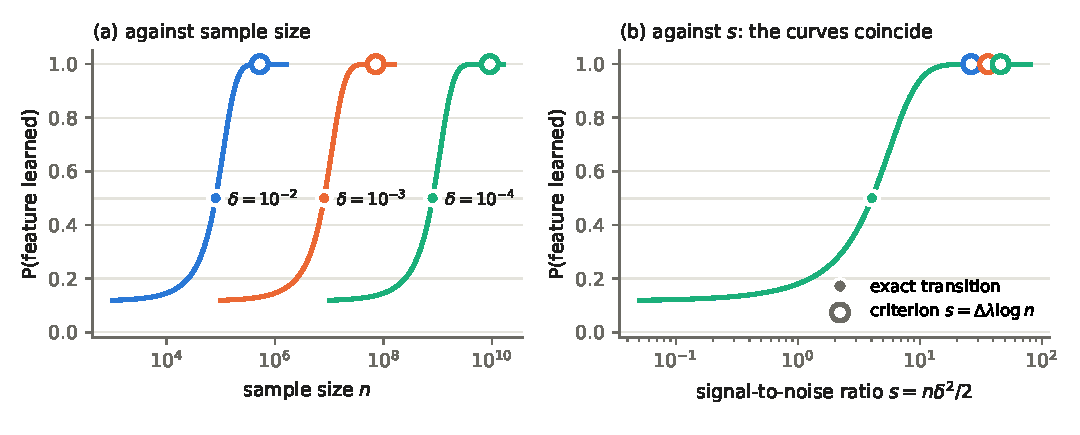
\includegraphics[width=\linewidth]{figures/fig1_headline.pdf}
\caption{Posterior probability that more than half of the feature is fitted, for $f_w(x)=a\,b^\top x$ with $M=5$, computed exactly from Eq.~\eqref{eq:toyZ}. Each curve is one truth of strength $\delta$. Filled dots: exact transition. Open circles: Eq.~\eqref{eq:rule}. (a) Against $n$. (b) Against $s=n\delta^2/2$, where the curves coincide.}
\label{fig:headline}
\end{figure}

\paragraph{Why the criterion fails.} \status{heuristic}
For $1\ll s\ll n$, split Eq.~\eqref{eq:toyZ} by the size of the output weight.
At $\lvert a\rvert\ll n^{-1/2}$ the feature is ignored: free energy $\lambda_0\log n+s$.
At $\lvert a\rvert=O(1)$ it is fitted with all $M$ input weights held to within $n^{-1/2}$: free energy $\lambda_1\log n+O(1)$.
Comparing only these two regions reproduces Eq.~\eqref{eq:rule}.
The region $n^{-1/2}\ll\lvert a\rvert\ll1$ also fits the feature, with input weights of order one, next to the branch $\{a=0\}$ where the input weights are free.
Its free energy is $\lambda_0\log n+\Delta\lambda\log s+O(1)$, lower than the $\lvert a\rvert=O(1)$ region by $\Delta\lambda\log(n/s)$, and the posterior moves into it continuously as $s$ grows.
So the fitted phase has $c_\alpha=\Delta\lambda\log\delta^2+O(1)$: the dropped constant diverges and cancels the $\log n$.

\section{Reduced-rank regression}

Let $f_w(x)=ABx$ with $A\in\R^{N\times H}$, $B\in\R^{H\times M}$, standard Gaussian priors, isotropic inputs and truth $Cx$.
Write $q=\min(N,H)$, $S=\tfrac n2CC^\top$ and $R_n(C)=Z_n(C)/Z_n(0)$.
Integrating out $B$ gives \status{proved, exact}
\begin{equation}
  Z_n(C)=\E_A\!\left[\det(I_H+nA^\top A)^{-M/2}\exp\!\Big(-\tfrac n2\operatorname{tr}\big[CC^\top(I_N+nAA^\top)^{-1}\big]\Big)\right].
  \label{eq:reduction}
\end{equation}
In singular-value coordinates of $A$ this splits into strata $j=0,\dots,q$ with exponents $\lambda_j=\tfrac12[jM+(H-j)(N-j)]$; $\lambda_0=\min_j\lambda_j$ is attained at $j_*$~\cite{AW05}.
The stratum $j_*$ contributes the angular factor
\begin{equation}
  \Phi_{j}(S)=\E_{U}\,\E_{V}\exp\!\big[-\tfrac n2\lVert(I-P_U)\,C\,(I-P_V)\rVert_F^2\big],
  \label{eq:Phi}
\end{equation}
with $U$ a Haar-random $j$-frame in $\R^N$ and $V$ a Haar-random $(H-j)$-frame in $\R^M$.
For rank-one $C$, $\Phi_j=\hypF22(\tfrac{N-j}2,\tfrac{M-H+j}2;\tfrac N2,\tfrac M2;-s)$ with $s=n\lVert C\rVert_F^2/2$.

\begin{theorem}[\status{proved}; \file{proof_B9}, Thm.~5]
If $j_*$ is unique, there are constants $C_0,c_0,n_0,\gamma>0$, depending on $N,H,M$ only, such that
\begin{equation}
  \big\lvert\log R_n(C)-\log\Phi_{j_*}(S)\big\rvert\le C_0\big(\lVert C\rVert_F^{2\gamma}+n^{-\gamma/2}\big)
  \label{eq:thm}
\end{equation}
for all $n\ge n_0$ and all $C$ of any rank with $\lVert C\rVert_F\le c_0$, where $\gamma=\tfrac13\min(1,\lambda_{j_*+1}-\lambda_{j_*},\lambda_{j_*-1}-\lambda_{j_*})$.
\end{theorem}

The proof bounds the dominant-stratum integrand above and below by factorised integrals whose ratio tends to one.
The bound is uniform in $s$: it covers $s\to0$, $s=O(1)$ and $s\to\infty$ with $s\le c_0^2n/2$.
So $-\log\Phi_{j_*}$ is the scaling function of $F_n(C)-F_n(0)$.
The error vanishes in the joint small-signal, large-$n$ limit, not at fixed nonzero $C$.

Its large-$s$ exponent equals Aoyagi and Watanabe's jump $\lambda(1)-\lambda(0)$ for rank-one $C$~\cite{AW05}.
I derive this independently from Eq.~\eqref{eq:Phi}; it agrees in exact arithmetic for all $8000$ triples with $N,H,M\le20$ \status{numerical}.
For rank-one truths, $F_n(C)=\lambda_0\log n+\Delta\lambda\log(1+s)+O(\log\log n)$ uniformly in $\lVert C\rVert_F\le c_0$.

\paragraph{Ties.} \status{proved, \file{proofs/proof_B9.pdf}, Thm.~9}
Two strata tie ($m_0=2$) exactly when $N+H+M$ is odd and $N,H,M$ satisfy strict triangle inequalities.
For rank-one $C$,
\begin{equation}
  R_n=\Phi(s)\,\frac{\log\frac n{1+s}+O(1)}{\log n+O(1)},\qquad 0\le s\le n/2 .
  \label{eq:tie}
\end{equation}
The multiplicity is paid as $\log\log(n/s)$.
At fixed $s$ the extra factor is $1+O(1/\log n)$; for $s=n^\theta$ it tends to $1-\theta$.

\section{Where the transition sits}

Table~\ref{tab:locations} collects transition locations \status{numerical}.
In every case the transition sits at an $n$-independent $s$ of order one, while Eq.~\eqref{eq:rule} grows with $\log n$.

\begin{table}[h]
\centering
\begin{tabular}{lcc}
\toprule
Model, $n$ & transition $s$ & Eq.~\eqref{eq:rule} \\
\midrule
$a\,b^\top x$, $M=5$, noise-free, all $n$ & $4.04$ & $18.4$--$36.8$ \\
$(3,1,3)$, noise-free, $5{\times}10^{4}$, $5{\times}10^{8}$ & $2.72$, $2.61$ & $10.9$, $20.1$ \\
$(8,1,8)$, noise-free, $2{\times}10^{5}$, $2{\times}10^{9}$ & $8.12$, $8.01$ & $42.0$, $74.2$ \\
$(2,1,2)$ tie, noise-free, $10^{4}$, $10^{8}$, $10^{32}$ & $1.75763$, $1.64693$, $1.57366$ & $4.6$, $9.2$, $36.8$ \\
$(2,1,3)$, sampled data, $10^{2}$, $10^{4}$, $10^{8}$ & $2.84$, $2.74$, $2.73$ & $4.6$--$18.4$ \\
\bottomrule
\end{tabular}
\caption{Transition location: the $s$ at which the window probability reaches $\tfrac12$ (for $a\,b^\top x$, the fitted fraction above $\tfrac12$). Triples are RRR $(N,H,M)$. Sampled data: mean over 64 data sets. The tie row is reproduced by \file{review_checks/check_calculations.py}, stable under grid doubling to better than $10^{-11}$.}
\label{tab:locations}
\end{table}

In the tie case the transition drifts slowly, from $2.03$ at $n=10^2$ to $1.557$ at $n=10^{128}$.
A fit $s_\infty+a/\log n+b/\log^2n$ gives $s_\infty\approx1.551$ \status{numerical}.
This drift is consistent with the $1/\log n$ correction in Eq.~\eqref{eq:tie}; the evidence-ratio theorem alone does not prove convergence of the window crossing.

The tie factor also accounts for the constant of the fitted phase.
Fitting it against $\log\delta^2$ without the factor gives slope $0.62$; with it, $0.507$ for $n\ge10^4$, against the predicted $\Delta\lambda=\tfrac12$ \status{numerical}.

\paragraph{Sampled data.}
For models linear in finitely many features, the $w$-dependence of the likelihood enters only through the least-squares fit $\hat C$ and the empirical second-moment matrix $\hat\Sigma$.
The empirical evidence is Eq.~\eqref{eq:Z} evaluated at truth $\hat C$ in the metric $\hat\Sigma$, up to a factor independent of $w$ \status{proved, exact; checked to relative error $4\times10^{-15}$}.
Data noise therefore shifts the truth by $O(n^{-1/2})$, the same order as the features studied here.
The theorem covers the resulting full-rank $S$, but not the $O(n^{-1/2})$ distortion of the prior from replacing the identity metric by $\hat\Sigma$, so the sampled-data transitions are numerical.

\section{Temperature and the learning coefficient}

At inverse temperature $\beta$ the unlocalised posterior in this model has effective sample size $n\beta$ \status{exact, population posterior}, so a feature is resolved when $n\beta\delta^2=O(1)$.
Stochastic-gradient Langevin estimators of the local learning coefficient (LLC) sample a tempered posterior, by default at $\beta=1/\log n$~\cite{LFWMW23}.
A feature with $1\lesssim s\lesssim\log n$ is then learned by the $\beta=1$ posterior but not counted at the default temperature \status{heuristic}.

Exact tempered-posterior values for RRR at $n=10^6$ (Fig.~\ref{fig:beta}) show one step per feature at $n\beta\delta_i^2=O(1)$, with an overshoot of $10$--$20\%$ before each plateau \status{numerical}.
At $n\beta=6.8\times10^4$, the grid point closest to $n/\log n$, the estimate is $3.45$ for $(2,2,4)$ and $1.81$ for $(3,1,3)$, against $4.06$ and $2.59$ at $\beta=1$.
SGLD reproduces the exact values to within $0.015$.
A sweep in $\beta$ therefore reads off the feature strengths from the step positions, which makes quantitative the observation of Ref.~\cite{CM25} that $\beta$ sets the resolution of the LLC.
A local estimator around a trained parameter adds localisation and baseline subtraction, which this calculation does not include.

\begin{figure}[t]
\centering
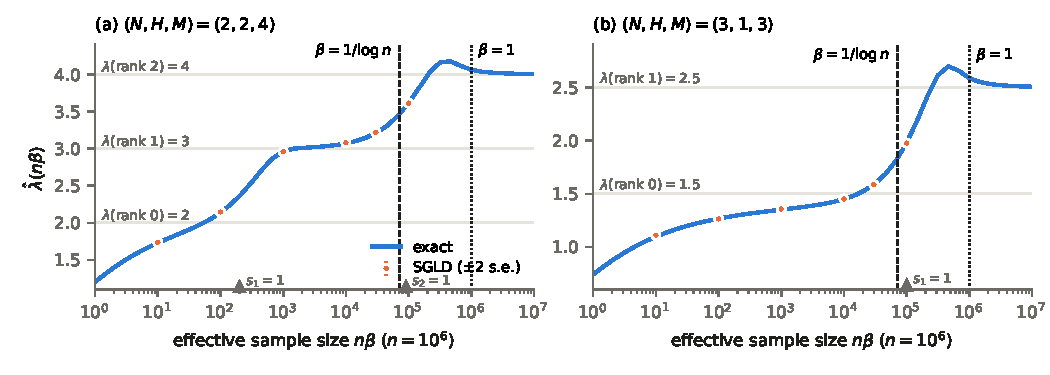
\includegraphics[width=\linewidth]{figures/fig4_beta.pdf}
\caption{Learning-coefficient estimate of the posterior tempered to effective sample size $n\beta$, RRR at fixed $n=10^6$, one sampled data set. Line: exact value; dots: SGLD. Gray lines: $\lambda$ for truths of rank $0,1,2$. Triangles: $s_i=n\beta\sigma_i^2/2=1$ for the singular values $\sigma_i$ of the least-squares fit. Dashed: default $\beta=1/\log n$; dotted: $\beta=1$. In (b) $\lambda_n(0)$ approaches $1.5$ slowly because $(3,1,3)$ is a tie case.}
\label{fig:beta}
\end{figure}

\section{Related work}

Detection of a weak signal at signal-to-noise ratio of order one is known in specific settings, including the one-unit model of Watanabe and Amari, for which the noisy evidence and generalisation coefficient are computed exactly~\cite{WA02,WA03}, and variational Bayesian matrix factorisation~\cite{NW07}.
What these notes add is the learning-coefficient bookkeeping across all widths of reduced-rank regression, the uniform bound of Eq.~\eqref{eq:thm}, the tie correction, and the identification of the dropped constant.

\section{Open questions}

\begin{itemize}
\item Whether the double-scaling form holds beyond reduced-rank regression, and under what geometric condition on the feature. I have partial results and will write them up separately.
\item The tie bound at rank two and higher.
\item A $\beta$-sweep in a small trained network with an independently measured weak feature, to test whether the steps of Fig.~\ref{fig:beta} survive localisation and sampler error.
\end{itemize}

\section*{Code}
The exact evaluator is \file{code/rrr.py}.
\file{review_checks/check_calculations.py} checks it against an independent integral (agreement $4\times10^{-10}$), reproduces the tie transitions in Table~\ref{tab:locations}, and runs a regression test for the sampled-data generator.

\begin{thebibliography}{99}
\bibitem{Wat09} S.~Watanabe, \emph{Algebraic Geometry and Statistical Learning Theory} (Cambridge University Press, 2009).
\bibitem{CLMWM23} Z.~Chen, E.~Lau, J.~Mendel, S.~Wei, and D.~Murfet, Dynamical versus Bayesian phase transitions in a toy model of superposition, arXiv:2310.06301.
\bibitem{LUWMW25} S.~Pepin Lehalleur \emph{et al.}, You are what you eat: AI alignment requires understanding how data shapes structure and generalisation, arXiv:2502.05475.
\bibitem{CHFM25} L.~Carroll, J.~Hoogland, M.~Farrugia-Roberts, and D.~Murfet, Dynamics of transient structure in in-context linear regression transformers, arXiv:2501.17745.
\bibitem{AW05} M.~Aoyagi and S.~Watanabe, Stochastic complexities of reduced rank regression in Bayesian estimation, Neural Netw.\ \textbf{18}, 924 (2005).
\bibitem{LFWMW23} E.~Lau, Z.~Furman, G.~Wang, D.~Murfet, and S.~Wei, The local learning coefficient: a singularity-aware complexity measure, arXiv:2308.12108.
\bibitem{CM25} Z.~Chen and D.~Murfet, Modes of sequence models and learning coefficients, arXiv:2504.18048.
\bibitem{WA02} S.~Watanabe and S.~Amari, The effect of singularities in a learning machine when the true parameters do not lie on such singularities, in \emph{Advances in Neural Information Processing Systems 15} (2003).
\bibitem{WA03} S.~Watanabe and S.~Amari, Learning coefficients of layered models when the true distribution mismatches the singularities, Neural Comput.\ \textbf{15}, 1013 (2003).
\bibitem{NW07} S.~Nakajima and S.~Watanabe, Variational Bayes solution of linear neural networks and its generalization performance, Neural Comput.\ \textbf{19}, 1112 (2007).
\end{thebibliography}
\end{document}
